%\documentclass[handout]{beamer}
\documentclass{beamer}

\mode<presentation>
{
\usetheme{default}
\usefonttheme[onlymath]{serif}
%\usetheme{Singapore}
%\usetheme{Warsaw}
%\usetheme{Malmoe}
% \useinnertheme{circles}
% \useoutertheme{infolines}
% \useinnertheme{rounded}

\setbeamercovered{transparent=5}
}

\usepackage[english]{babel}
\usepackage[latin1]{inputenc}
\usepackage{textpos,alltt,listings,multirow,ulem,siunitx}
\newcommand\hmmax{0}
\newcommand\bmmax{0}
\usepackage{bm}

% font definitions, try \usepackage{ae} instead of the following
% three lines if you don't like this look
\usepackage{mathptmx}
\usepackage[scaled=.90]{helvet}
%\usepackage{courier}
\usepackage[T1]{fontenc}
\usepackage{tikz}
\usetikzlibrary[shapes,shapes.arrows,arrows,shapes.misc,fit,positioning]

% \usepackage{pgfpages}
% \pgfpagesuselayout{4 on 1}[a4paper,landscape,border shrink=5mm]

\usepackage{slashbox,multirow,listings,booktabs}
\usepackage{xspace}
\makeatletter
\DeclareRobustCommand\onedot{\futurelet\@let@token\@onedot}
\def\@onedot{\ifx\@let@token.\else.\null\fi\xspace}
\def\eg{{e.g}\onedot} \def\Eg{{E.g}\onedot}
\def\ie{{i.e}\onedot} \def\Ie{{I.e}\onedot}
\def\cf{{c.f}\onedot} \def\Cf{{C.f}\onedot}
\def\etc{{etc}\onedot}
\def\vs{{vs}\onedot}
\def\wrt{w.r.t\onedot}
\def\dof{d.o.f\onedot}
\def\etal{{et al}\onedot}
\makeatother

\usepackage{tikz}
\usetikzlibrary[shapes,shapes.arrows,arrows,shapes.misc,fit,positioning]

\usepackage{siunitx}
\DeclareSIUnit\year{a}
\DeclareSIUnit\byte{B}
\sisetup{retain-unity-mantissa = false}

\usepackage{fancyvrb}
\usepackage{minted}
\newminted{c}{gobble=2}
\newminted{python}{gobble=2}
%\newmint[cverb]{c}{} 
\newcommand\cverb[1][]{\SaveVerb[%
    aftersave={\textnormal{\UseVerb[#1]{vsave}}}]{vsave}}
\newcommand\cfunc[1][]{\SaveVerb[%
    aftersave={\textnormal{\UseVerb[#1]{vsave}\texttt{()}}}]{vsave}}
\newcommand\pyverb[1][]{\SaveVerb[%
    aftersave={\textnormal{\UseVerb[#1]{vsave}}}]{vsave}}
\def\asm#1{{\tt #1}}
\def\code#1{{\tt #1}}
\def\shell#1{{\tt \$ #1}}

\newcommand\email[1]{{\href{mailto:#1}{\nolinkurl{#1}}}}

\newcommand{\II}{\mathcal{I}}
\newcommand{\C}{\mathbb{C}}
\newcommand{\D}{\mathcal{D}}
\newcommand{\EE}{\mathcal{E}}
\newcommand{\F}{\mathcal{F}}
\newcommand{\I}{\mathcal{I}}
\newcommand{\N}{\mathcal{N}}
\newcommand{\PP}{\mathcal{P}}
\newcommand\Ppc{\ensuremath{\mathsf P}}
\newcommand{\bigO}{\ensuremath{\mathcal{O}}}
\newcommand{\R}{\mathbb{R}}
\newcommand{\Rz}{\mathcal{R}}
\newcommand{\QQ}{\mathcal Q}
\newcommand{\VV}{\mathcal V}
\newcommand{\ASM}{\mathrm{ASM}}
\newcommand{\RASM}{\mathrm{RASM}}

\newcommand{\kb}{\tt}
\newcommand{\Pk}[1]{\ensuremath{P_{#1}}}
\newcommand{\Qk}[1]{\ensuremath{Q_{#1}}}
\newcommand{\Pkdisc}[1]{\ensuremath{P_{#1}^{\text{disc}}}}
\newcommand{\Qkdisc}[1]{\ensuremath{Q_{#1}^{\text{disc}}}}
\newcommand{\blue}{\textcolor{blue}}
\newcommand{\green}{\textcolor{green!70!black}}
\newcommand{\red}{\textcolor{red}}
\newcommand{\brown}{\textcolor{brown}}
\newcommand{\cyan}{\textcolor{cyan}}
\newcommand{\magenta}{\textcolor{magenta}}
\newcommand{\yellow}{\textcolor{yellow}}
\newcommand{\mini}{\mathop{\rm minimize}}
\newcommand{\st}{\mbox{subject to }}
\newcommand{\lap}{\Delta}
\newcommand{\grad}{\nabla}
\newcommand\mtab{\hspace{\stretch{1}}}
\newcommand\ud{\,\mathrm{d}}
\newcommand\bslash{{$\backslash$}}
\newcommand\half{{\frac 1 2}}
\newcommand{\abs}[1]{\left\lvert #1 \right\rvert}
\newcommand{\bigabs}[1]{\big\lvert #1 \big\rvert}
\newcommand{\norm}[1]{\left\lVert #1 \right\rVert}
\newcommand\oneitem[1]{\begin{itemize} \item #1 \end{itemize}}
\newcommand\pfrak{{\mathfrak p}}
\newcommand\nfrak{{\mathfrak n}}
\newcommand\ff{\bm f}
\newcommand\mm{\bm m}
\newcommand\nn{\bm n}
\newcommand\uu{\bm u}
\newcommand\vv{\bm v}
\newcommand\ww{\bm w}
\newcommand\DD{D}
\newcommand{\tcolon}{\!:\!}
\DeclareMathOperator{\sgn}{sgn}
\DeclareMathOperator{\card}{card}
\DeclareMathOperator{\trace}{tr}
\DeclareMathOperator{\erf}{erf}
\DeclareMathOperator{\sspan}{span}
\renewcommand{\bar}{\overline}
% \DeclareMathOperator{\divergence}{div}
% \renewcommand\div\divergence
\renewcommand{\div}{{\nabla \cdot}}
\newcommand\spliceop{\leftrightsquigarrow}
\newcommand\splice[5]{{#1} \overset{#5}{\underset{#3,#4}{\leftrightsquigarrow}} {#2}}
\newcommand{\ip}[2]{{\left\langle #1, #2 \right\rangle}}
\newcommand{\Linfty}{{L^\infty}}

% Dimensionless numbers
\newcommand{\Peclet}{{\mathrm{Pe}}}
\newcommand{\Reynolds}{{\mathrm{Re}}}
\newcommand{\Rayleigh}{{\mathrm{Ra}}}
\newcommand{\Mach}{{\mathrm{Ma}}}
\newcommand{\Prandtl}{{\mathrm{Pr}}}
\newcommand{\Grashof}{{\mathrm{Gr}}}

\newcommand{\PETSc}{{PETSc}}
\newcommand{\Dohp}{{Dohp}}
\newcommand\libmesh{\texttt{libMesh}}
\newcommand\dealii{\texttt{Deal.II}}
\newcommand\MatMult{\cverb|MatMult|}
\newcommand\MatSolve{\cverb|MatSolve|}
\newcommand{\secref}[1]{{Section~\ref{#1}}}
\newcommand{\chapref}[1]{{Chapter~\ref{#1}}}
\newcommand{\figref}[1]{{Figure~\ref{#1}}}
\newcommand{\tabref}[1]{{Table~\ref{#1}}}
\newcommand\AIJ{{\cverb|AIJ|}}
\newcommand\AIJInode{\cverb|AIJ|/\cverb|Inode|}
\newcommand\BAIJ[1][]{\ifthenelse{\equal{#1}{}}{\cverb|BAIJ|}{\ensuremath{\cverb|BAIJ|(#1)}}}
\newcommand\SBAIJ[1][]{\ifthenelse{\equal{#1}{}}{\cverb|SBAIJ|}{\ensuremath{\cverb|SBAIJ|(#1)}}}
\newcommand\todo[1]{{\color{red}\bf [TODO: #1]}}
\newcommand\tf[1]{\hat{#1}}     % test functions


\title{Scalable Implicit Methods for Free Surface Flows in Glaciology}
\subtitle{Scalable Ice-sheet Solvers and Infrastructure for Petascale, High-resolution, Unstructured Simulations (SISIPHUS) \\
DOE ASCR ISICLES}

\author{Jed Brown\inst{1,2}, Iulian Grindeanu\inst{1}, Dmitry Karpeev\inst{1}, Barry F. Smith\inst{1}, and Timothy J. Tautges\inst{1}}


% - Use the \inst command only if there are several affiliations.
% - Keep it simple, no one is interested in your street address.
\institute
{
  \inst{1}{Argonne National Laboratory} \\
  \inst{2}{ETH Z\"urich}
}

\date{2011-07-20}

% This is only inserted into the PDF information catalog. Can be left
% out.
\subject{Talks}


% If you have a file called "university-logo-filename.xxx", where xxx
% is a graphic format that can be processed by latex or pdflatex,
% resp., then you can add a logo as follows:

% \pgfdeclareimage[height=0.5cm]{university-logo}{university-logo-filename}
% \logo{\pgfuseimage{university-logo}}



% Delete this, if you do not want the table of contents to pop up at
% the beginning of each subsection:
% \AtBeginSubsection[]
% {
% \begin{frame}<beamer>
% \frametitle{Outline}
% \tableofcontents[currentsection,currentsubsection]
% \end{frame}
% }

\AtBeginSection[]
{
\begin{frame}<beamer>
\frametitle{Outline}
\tableofcontents[currentsection]
\end{frame}
}

% If you wish to uncover everything in a step-wise fashion, uncomment
% the following command:

%\beamerdefaultoverlayspecification{<+->}

\begin{document}
\lstset{language=C}
\normalem

\begin{frame}
\titlepage
\end{frame}

\section{Objectives}
\begin{frame}
  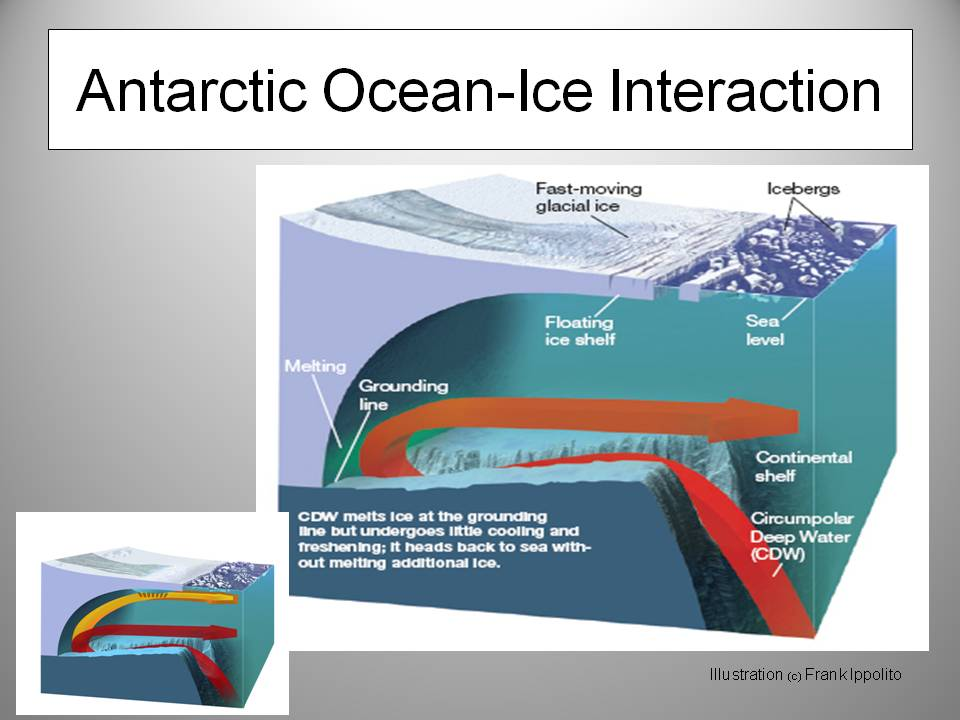
\includegraphics[width=\textwidth]{figures/GroundingLine/NaturalHistory2008} \\
  \vspace{-.5em}
  {\tiny Bindschadler 2008}
\end{frame}

\begin{frame}
  \begin{block}{Glaciology and society}
    \begin{itemize}
    \item Quantitative analysis of ice dynamics in changing climate
    \item Inversion to determine current state
    \item Stability and sensitivity, mostly at grounding line
    \item Prediect sea level rise as a function of sea surface temperature [energy policy]
    \end{itemize}
  \end{block}
  \begin{block}{Our efforts}
    \begin{itemize}
    \item Unstructured meshing, geometric models of boundaries
    \item Fully implicit formulations to enable analysis
    \item Implicit solver components
      \begin{itemize}
      \item saddle points, anisotropy, heterogeneity, transport
      \item composability and multi-physics coupling
      \end{itemize}
    \item High order accuracy and high throughput
    \item Adjoints using restricted AD
    \end{itemize}
  \end{block}
\end{frame}

\section{Some opinionated commentary}
\begin{frame}[shrink=5]{Bathymetry and stickyness distribution}
  \begin{itemize}
  \item Bathymetry:
    \begin{itemize}
    \item Aspect ratio $\epsilon = [H]/[x] \ll 1$
    \item Need surface \emph{and} bed slopes to be small
    \end{itemize}
  \item Stickyness distribution:
    \begin{itemize}
    \item Limiting cases of plug flow versus vertical shear
    \item Stress ratio: $\lambda = [\tau_{xz}]/[\tau_{\text{membrane}}]$
    \item Discontinuous: frozen to slippery transition at ice stream margins
    \end{itemize}
  \item Standard approach in glaciology: \\
    Taylor expand in $\epsilon$ and sometimes $\lambda$, drop higher order terms.
    \begin{itemize}
    \item[$\lambda \gg 1$] Shallow Ice Approximation (SIA), no horizontal coupling
    \item[$\lambda \ll 1$] Shallow Shelf Approximation (SSA), 2D elliptic solve in map-plane
    \item Hydrostatic and various hybrids, 2D or 3D elliptic solves
    \end{itemize}
  \item \alert{\large Bed slope is discontinuous and of order 1.}
    \begin{itemize}
    \item Taylor expansions no longer valid
    \item Numerics require high resolution, subgrid parametrization, short time steps
    \item Still get low quality results in the regions of most interest.
    \end{itemize}
  \item \alert{\large Basal sliding parameters are discontinuous.}
  \end{itemize}
\end{frame}

\begin{frame}{Textbook multigrid efficiency}
  \includegraphics[width=\textwidth]{figures/THI/x-80km-m16p2l6-ew} \\
  Grid-sequenced Newton-Krylov solution of test $X$.  The solid lines denote nonlinear iterations, and the dotted lines with $\times$ denote linear residuals.
\end{frame}

\begin{frame}{Strong scaling on Shaheen}
  \centering
  \includegraphics[width=\textwidth]{figures/THI/shaheen-strong} \\
  Strong scaling on Shaheen for different size coarse levels problems and different coarse level solvers.
  The straight lines on the strong scaling plot have slope $-1$ which is optimal.
\end{frame}



\section{Conservative steady-state energy transport}
\newcommand\smallterm[1]{{\color{gray} #1}}
\begin{frame}{Conservative two-phase formulation}
  Find momentum density $\rho\uu$, pressure $p$, and total energy density $E$:
  \begin{gather*}
    (\rho\uu)_t + \div (\smallterm{\rho\uu\otimes\uu} - \eta D\uu_i + p\bm 1) - \rho \bm g = 0 \\
    \rho_t + \div \rho\uu = 0 \\
    E_t + \div \big((E+p)\uu - k_T\nabla T - k_\omega\nabla\omega \big) - \eta D\uu_i\tcolon D\uu_i - \smallterm{\rho\uu\cdot\bm g} = 0
  \end{gather*}
\begin{itemize}
\item Solve for density $\rho$, ice velocity $\uu_i$, temperature $T$, and melt fraction $\omega$ using constitutive relations.
  \begin{itemize}
  \item Simplified constitutive relations can be solved explicitly.
  \item Temperature, moisture, and strain-rate dependent rheology $\eta$.
  \item High order FEM, typically $Q_3$ momentum \& energy, SUPG (yuck).
  \end{itemize}
\item DAEs solved implicitly after semidiscretizing in space.
\item Newton solver converges quadratically.
\item Thermocoupled steady state in one nonlinear solve
  \begin{itemize}
  \item no time stepping needed, total cost similar to 3 semi-implicit steps
  \item useful for inverse problems and stability analysis
  \end{itemize}
\item (Somewhat) robust preconditioning using nested field-split
\end{itemize}
\end{frame}

\begin{frame}{Block on inclined plate, nominal $\Reynolds = 0.24$, $\Peclet = 120$}
  \begin{columns}
    \begin{column}{0.5\textwidth}
      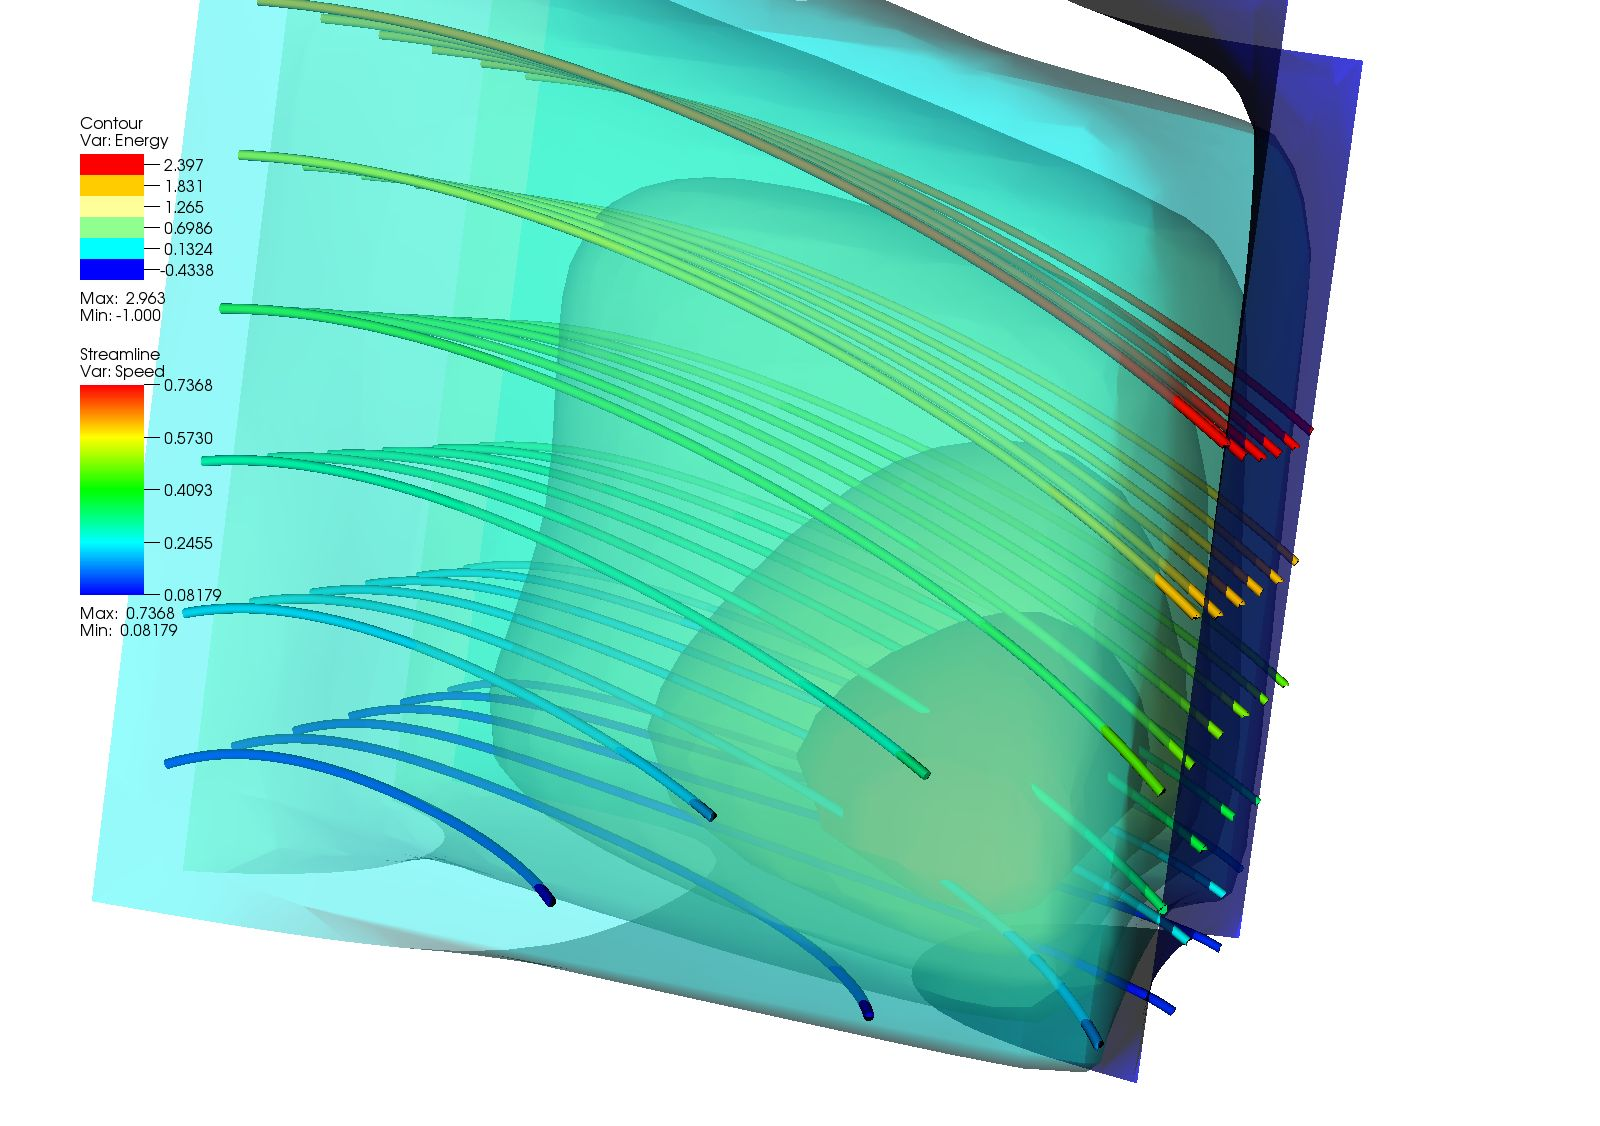
\includegraphics[width=1.3\textwidth]{figures/VHTNondimEnergy} \\
      Contours of Energy, melt fraction up to 15\%, density ratio 2.
    \end{column}
    \begin{column}{0.5\textwidth}
      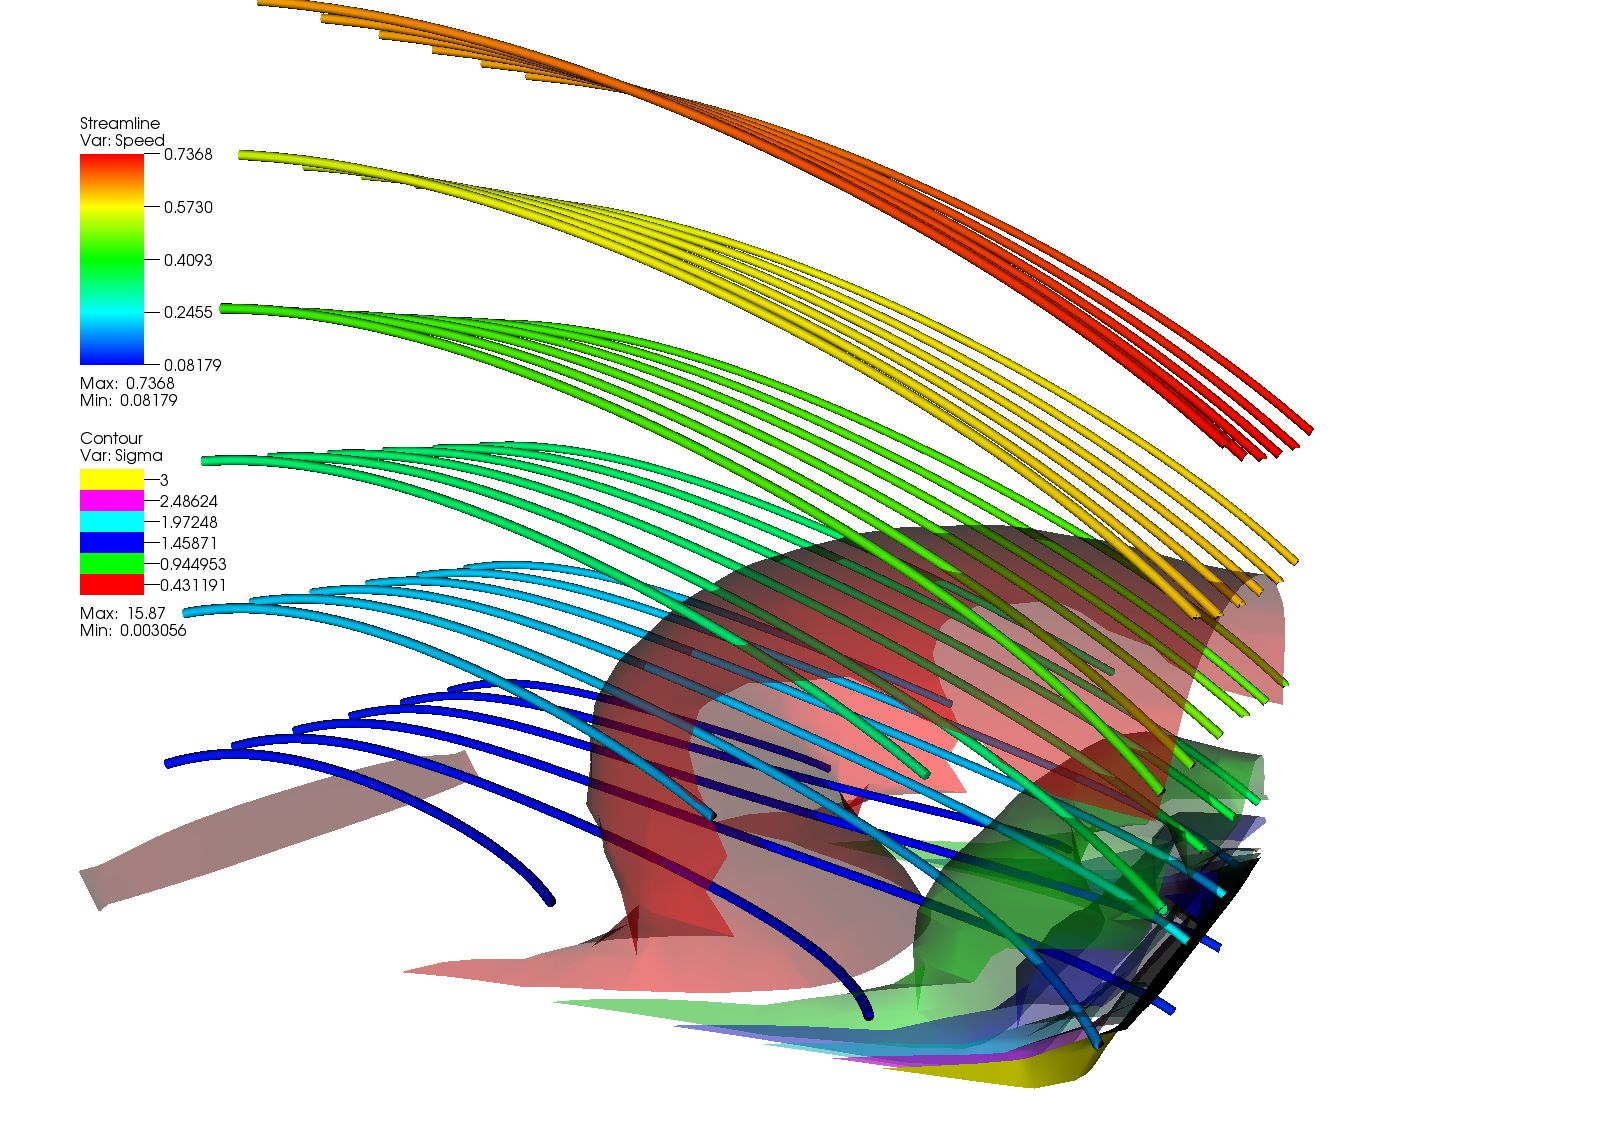
\includegraphics[width=1.3\textwidth]{figures/VHTNondimSigma} \\
      Contours of viscous heat production, $1/r$ singularity at corners.
    \end{column}
  \end{columns}
\end{frame}

\begin{frame}{Relative effect of the blocks}
  \begin{equation*}\label{eq:vhtblock}
    J =
    \begin{pmatrix}
      J_{uu} & J_{up} & J_{uE} \\
      J_{pu} & 0 & 0 \\
      J_{Eu} & J_{Ep} & J_{EE}
    \end{pmatrix} .
  \end{equation*}
  \begin{itemize}
  \item[$J_{uu}$] Viscous/momentum terms, nearly symmetric, variable coefficionts, anisotropy from Newton.
  \item[$J_{up}$] Weak pressure gradient, viscosity dependence on pressure (small), gravitational contribution (pressure-induced density variation).
    Large, nearly balanced by gravitational forcing.
  \item[$J_{uE}$] Viscous dependence on energy, very nonlinear, not very large.
  \item[$J_{pu}$] Divergence (mass conservation), nearly equal to $J_{up}^T$.
  \item[$J_{Eu}$] Sensitivity of energy on momentum, mostly advective transport.
    Large in boundary layers with large thermal/moisture gradients.
  \item[$J_{Ep}$] Thermal/moisture diffusion due to pressure-melting, $\uu \cdot \nabla$.
  \item[$J_{EE}$] Advection-diffusion for energy, very nonlinear at small regularization.
    Advection-dominated except in boundary layers and stagnant ice, often balanced in vertical.
  \end{itemize}
\end{frame}

\begin{frame}{How much nesting?}
  \begin{columns}
    \begin{column}{0.5\textwidth}
      \begin{equation*}
        P_1 =
        \begin{pmatrix}
          J_{uu} & J_{up} & J_{uE} \\
          0 & B_{pp} & 0 \\
          0 & 0 & J_{EE} \\
        \end{pmatrix}
      \end{equation*}
      \begin{itemize}
      \item $B_{pp}$ is a mass matrix in the pressure space weighted by inverse of kinematic viscosity.
      \item Elman, Mihajlovi\'c, Wathen, JCP 2011 for non-dimensional isoviscous Boussinesq.
      \item Works well for non-dimensional problems on the cube, not for realistic parameters.
      \end{itemize}
    \end{column}
    \begin{column}{0.5\textwidth}
      \begin{equation*}
        P =
        \begin{bmatrix}
          \begin{pmatrix}
            J_{uu} & J_{up} \\
            J_{pu} & 0
          \end{pmatrix} & \\
          \begin{pmatrix}
            J_{Eu} & J_{Ep}
          \end{pmatrix}
          & J_{EE}
        \end{bmatrix}
      \end{equation*}
      \begin{itemize}
      \item Inexact inner solve using upper-triangular with $B_{pp}$ for Schur.
      \item Another level of nesting.
      \item GCR tolerant of inexact inner solves.
      \item Outer converges in 1 or 2 iterations.
      \end{itemize}
    \end{column}
  \end{columns}
  \begin{itemize}
  \item Low-order preconditioning full-accuracy unassembled high order operator.
  \item Build these on command line with PETSc \cverb|PCFieldSplit|.
  \end{itemize}
\end{frame}


\begin{frame}[shrink=5]{Everything is better as a smoother (sometimes)}
  \begin{block}{Block preconditioners work alright, but\ldots}
    \begin{itemize}
    \item nested iteration requires more dot products
    \item more iterations: coarse levels don't ``see'' each other
    \item finer grained kernels: lower arithmetic intensity, even more limited by memory bandwidth
    \end{itemize}
  \end{block}
  \begin{block}{Coupled multigrid}
    \begin{itemize}
    \item need compatible coarsening
      \begin{itemize}
      \item can do algebraically (Adams 2004) but would need to assemble
      \end{itemize}
    \item stability issues for lowest order $Q_1-P_0^{\text{disc}}$
      \begin{itemize}
      \item Rannacher-Turek looks great, but no discrete Korn's inequality
      \end{itemize}
    \item coupled ``Vanka'' smoothers difficult to implement with high performance, especially for FEM
    \item block preconditioners as smoothers reuse software better
    \item one level by reducing order for the coarse space, more levels need non-nested geometric MG or go all-algebraic and pay for matrix assembly and setup
    \end{itemize}
  \end{block}
\end{frame}

\begin{frame}
  \centering
  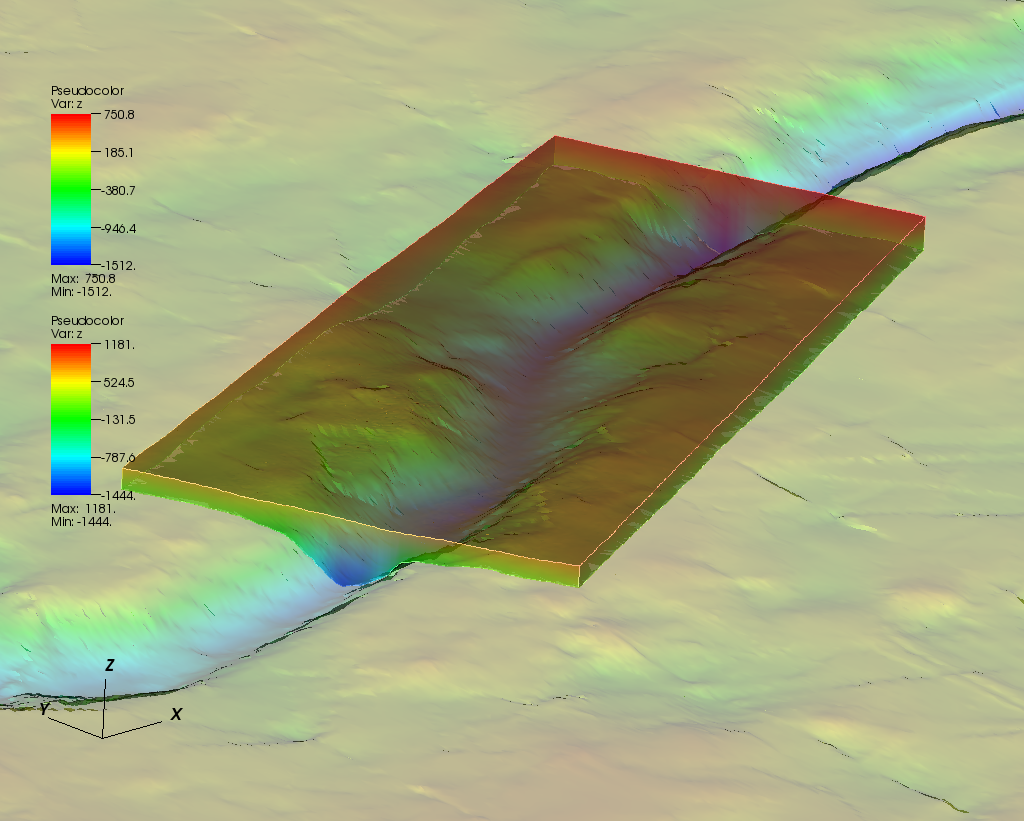
\includegraphics[width=\textwidth]{figures/jakotransparent}
\end{frame}

\begin{frame}
  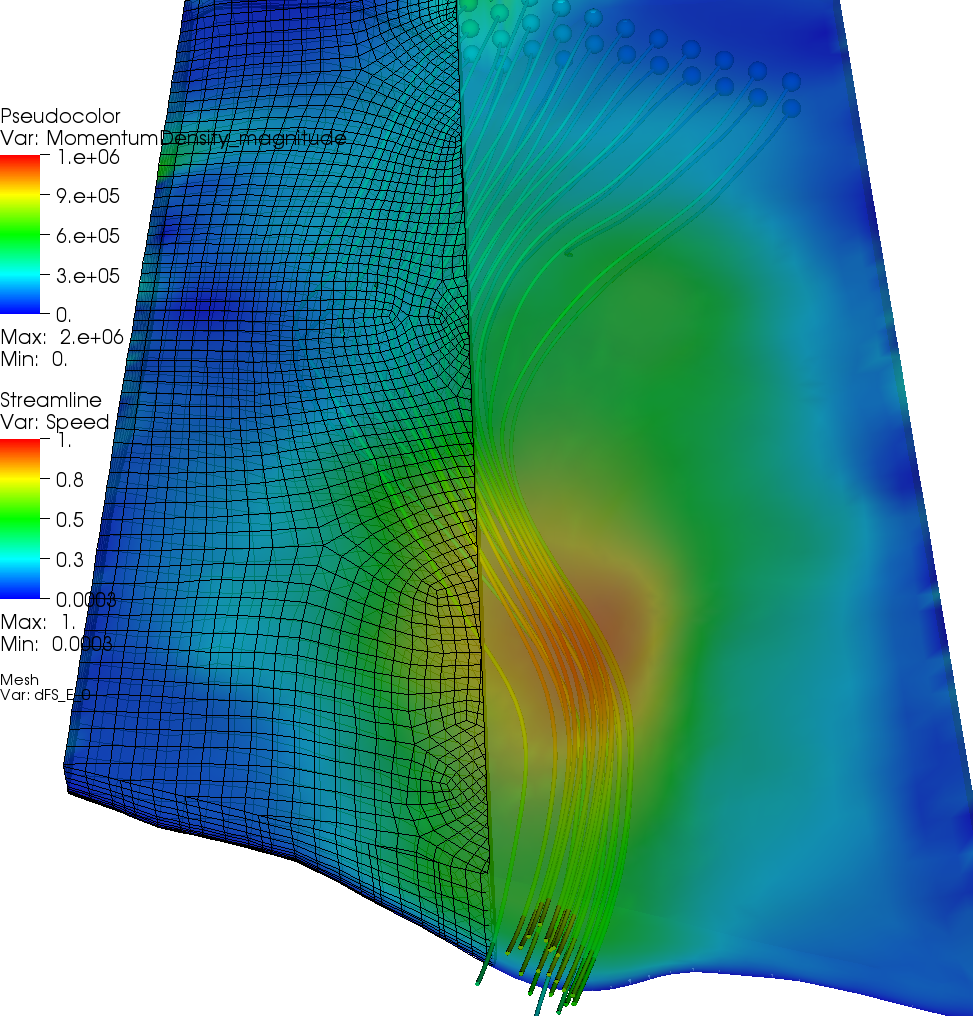
\includegraphics[width=\textwidth]{figures/VHT/TopViewStreamline}
\end{frame}

\begin{frame}
  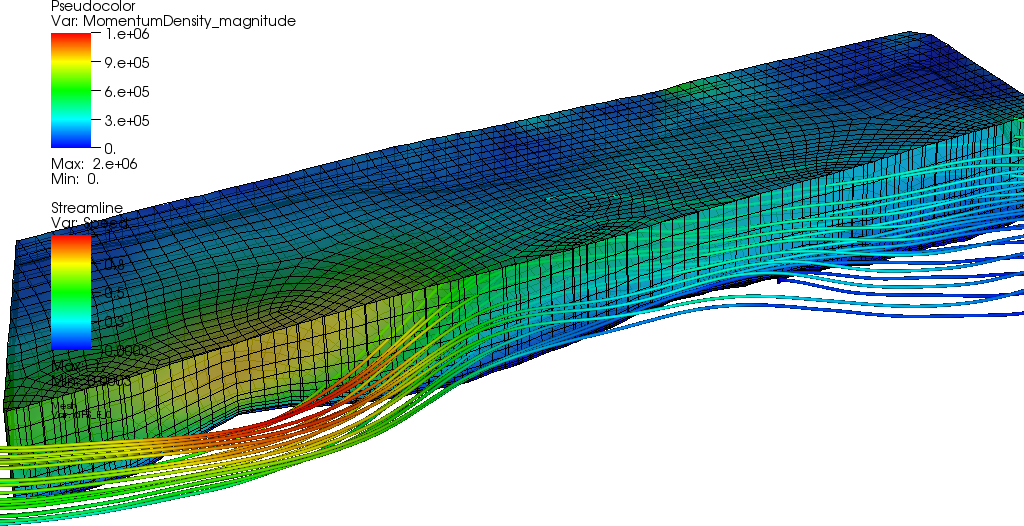
\includegraphics[width=0.9\textwidth]{figures/VHT/JakoSideMomentum} \\
  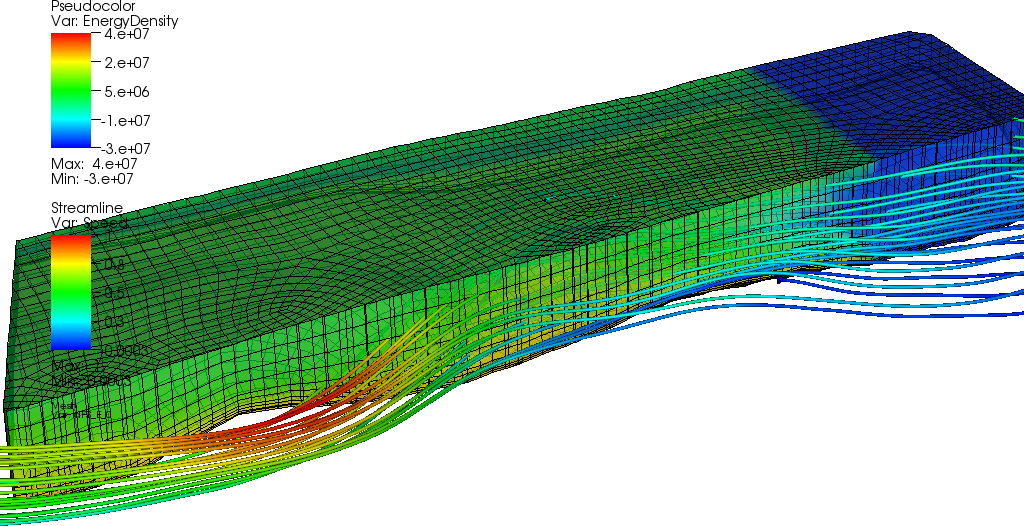
\includegraphics[width=0.9\textwidth]{figures/VHT/JakoSideEnergy}
\end{frame}


\section{Code verification}
\begin{frame}[fragile,shrink=5]{Symbolic form of large-deformation elasticity}
  Find displacement vector $\uu$ such that:
  \begin{equation*}
    \int_\Omega \nabla \vv \tcolon \Pi = 0,\quad \forall \vv
  \end{equation*}
  where
  \begin{align*}
    F   & = I - \nabla \uu                &  & \text{Deformation gradient}  \\
    E   & = (F^T F - I)/2                 &  & \text{Green-Lagrange tensor} \\
    S   & = \lambda (\trace E) I + 2\mu E &  & \text{Second Piola-Kirchoff tensor} \\
\uncover<2>{\alert{S}   & \alert{ = \lambda (J^2 - I) C^{-1} + \mu (I - C^{-1})}} & & \uncover<2>{\text{Neo-Hookean material, } (C = F^T F)} \\
    \Pi & = F \cdot S                     &  & \text{First Piola-Kirchoff tensor}
  \end{align*}
  \vspace{-0.8em}
\begin{pythoncode}
  def weak_form(u, du, v, dv):
    I = eye(3)                      # Identity tensor
    F = I - du                      # Deformation gradient
    E = (F.T*F - I)/2               # Green-Lagrange tensor
    S = lmbda*E.trace()*I + 2*mu*E  # Second Piola-Kirchoff tensor
    Pi = F * S                      # First Piola-Kirchoff tensor
    return dv.dot(Pi)
\end{pythoncode}
\end{frame}

\begin{frame}[fragile]{Manufactured solution}
  \begin{itemize}
  \item Choose a solution $\uu_{\text{exact}}$ with rich derivatives
  \begin{pythoncode}
  def solution(x,y,z, a,b,c):
    return Matrix([cos(x) * exp(y) * z + sin(z),
                   sin(x) * tanh(y) + x * cosh(z),
                   exp(x) * sinh(y) + y * log(1+z**2)])
  \end{pythoncode}
  \item Apply strong-form nonlinear differential operator symbolically
    to define
    \[ f(x,y,z) = \nabla\cdot \Pi(\nabla \uu_{\text{exact}}) \]
  \item Solve finite element problem for $\uu_h$
    \begin{equation*}
      \int_\Omega \nabla \vv \tcolon \Pi(\nabla \uu_h) = \int v\cdot f(x,y,z),\quad \forall \vv
    \end{equation*}
  \item Compute norms of $\uu_h - \uu_{\text{exact}}$.
  \end{itemize}
\end{frame}

\begin{frame}{Manufactured solution}
  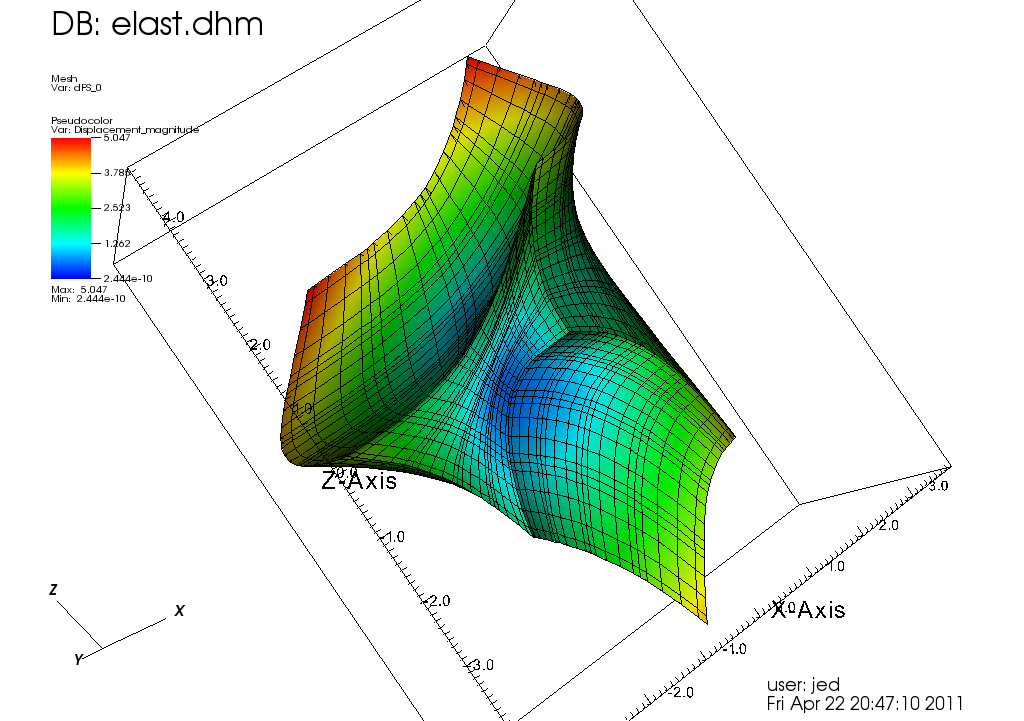
\includegraphics[width=\textwidth]{figures/elast-b4q5} \\
\end{frame}

\begin{frame}[shrink=30]{Convergence rates}
  \begin{tabular}{lrr rr rr rr rr}
    \toprule
    & & & \multicolumn{2}{c}{$\norm{\uu_h - \uu}_2$} & \multicolumn{2}{c}{$\norm{\uu_h - \uu}_\infty$}
    & \multicolumn{2}{c}{$\norm{\nabla\uu_h - \nabla\uu}_2$} & \multicolumn{2}{c}{$\norm{\nabla\uu_h - \nabla\uu}_\infty$} \\
    \cmidrule(r){4-5} \cmidrule(lr){6-7} \cmidrule(lr){8-9} \cmidrule(l){10-11}
    \multicolumn{2}{c}{Mesh} & \# Nodes & Error & \bigO & Error & \bigO & Error & \bigO & Error & \bigO \\
    \midrule % output below is generated with verif.py in this directory
$Q_1$ & $1^3$ & 8 & 1.79e+00 & --- & 6.50e-01 & --- & 3.70e+00 & --- & 1.08e+00 & --- \\
$Q_1$ & $2^3$ & 27 & 5.49e-01 & 1.71 & 3.40e-01 & 0.93 & 1.61e+00 & 1.20 & 6.92e-01 & 0.64 \\
$Q_1$ & $4^3$ & 125 & 1.53e-01 & 1.84 & 1.26e-01 & 1.43 & 8.01e-01 & 1.01 & 4.51e-01 & 0.62 \\
$Q_1$ & $8^3$ & 729 & 3.94e-02 & 1.96 & 3.73e-02 & 1.76 & 3.98e-01 & 1.01 & 2.81e-01 & 0.68 \\
$Q_1$ & $16^3$ & 4913 & 9.95e-03 & 1.99 & 1.01e-02 & 1.88 & 1.98e-01 & 1.01 & 1.57e-01 & 0.84 \\
$Q_1$ & $32^3$ & 35937 & 2.49e-03 & 2.00 & 2.61e-03 & 1.95 & 9.92e-02 & 1.00 & 8.32e-02 & 0.92\\
% \midrule
% $Q_2$ & $1^3$ & 27 & 2.44e-01 & --- & 1.82e-01 & --- & 9.48e-01 & --- & 4.60e-01 & --- \\
% $Q_2$ & $2^3$ & 125 & 3.71e-02 & 2.72 & 4.47e-02 & 2.03 & 2.86e-01 & 1.73 & 1.54e-01 & 1.58 \\
% $Q_2$ & $4^3$ & 729 & 4.48e-03 & 3.05 & 6.23e-03 & 2.84 & 6.94e-02 & 2.04 & 4.34e-02 & 1.83 \\
% $Q_2$ & $8^3$ & 4913 & 5.60e-04 & 3.00 & 9.31e-04 & 2.74 & 1.74e-02 & 2.00 & 1.29e-02 & 1.75 \\
% $Q_2$ & $16^3$ & 35937 & 7.01e-05 & 3.00 & 1.23e-04 & 2.92 & 4.34e-03 & 2.00 & 3.52e-03 & 1.87\\
\midrule
$Q_3$ & $1^3$ & 64 & 4.14e-02 & --- & 2.71e-02 & --- & 2.90e-01 & --- & 1.63e-01 & --- \\
$Q_3$ & $2^3$ & 343 & 2.06e-03 & 4.33 & 2.06e-03 & 3.72 & 2.39e-02 & 3.60 & 1.14e-02 & 3.84 \\
$Q_3$ & $4^3$ & 2197 & 1.81e-04 & 3.51 & 2.06e-04 & 3.32 & 4.23e-03 & 2.50 & 2.88e-03 & 1.98 \\
$Q_3$ & $8^3$ & 15625 & 1.22e-05 & 3.89 & 1.87e-05 & 3.46 & 5.79e-04 & 2.87 & 5.84e-04 & 2.30\\
\midrule
$Q_5$ & $1^3$ & 216 & 3.76e-03 & --- & 2.90e-03 & --- & 4.69e-02 & --- & 3.16e-02 & --- \\
$Q_5$ & $2^3$ & 1331 & 7.58e-05 & 5.63 & 5.92e-05 & 5.61 & 1.62e-03 & 4.86 & 1.05e-03 & 4.91 \\
$Q_5$ & $4^3$ & 9261 & 7.33e-07 & 6.69 & 6.61e-07 & 6.48 & 2.59e-05 & 5.97 & 1.76e-05 & 5.90\\
% \midrule
% $Q_7$ & $1^3$ & 512 & 4.46e-04 & --- & 3.59e-04 & --- & 8.15e-03 & --- & 5.83e-03 & --- \\
% $Q_7$ & $2^3$ & 3375 & 2.95e-06 & 7.24 & 2.95e-06 & 6.93 & 8.21e-05 & 6.63 & 6.05e-05 & 6.59 \\
% $Q_7$ & $4^3$ & 24389 & 7.65e-09 & 8.59 & 1.07e-08 & 8.11 & 4.09e-07 & 7.65 & 3.95e-07 & 7.26\\
\midrule
$Q_9$ & $1^3$ & 1000 & 5.81e-05 & --- & 5.04e-05 & --- & 1.42e-03 & --- & 1.05e-03 & --- \\
$Q_9$ & $2^3$ & 6859 & 6.27e-08 & 9.86 & 7.59e-08 & 9.38 & 1.63e-06 & 9.77 & 1.60e-06 & 9.36 \\
\bottomrule
  \end{tabular}
\end{frame}


\section{Coupling software}
\newcommand{\colorA}[1]{{\color{red} #1}}
\newcommand{\colorB}[1]{{\color{green!60!black} #1}}
\newcommand{\colorC}[1]{{\color{blue} #1}}
\newcommand{\colorD}[1]{{\color{magenta!70!black} #1}}
\newcommand{\colorE}[1]{{\color{cyan!70!black} #1}}
\newcommand{\colorF}[1]{{\color{yellow!60!black} #1}}
\newcommand{\colorG}[1]{{\color{red!50!white} #1}}

\begin{frame}{ALE form}
  After discretization in time ($\alpha \propto 1/\Delta t$) we have a Jacobian
  \begin{equation*}
    \begin{bmatrix}
      \colorA{A_{II}} & \colorA{A_{I\Gamma}}             &                       &                             &                     &   \\
      & \colorB{\alpha M_{\Gamma\Gamma}} &                       & \colorB{- N_{\Gamma\Gamma}} &                       &  \\
      \colorG{G_{II}}      & \colorG{G_{\Gamma I}} & \colorC{B_{II}}       & \colorC{B_{I\Gamma}}        & \colorC{C_{I}^T}    & \colorD{D_I} \\
      \colorG{G_{I\Gamma}} &        \colorG{G_{\Gamma\Gamma}}                          & \colorC{B_{\Gamma I}} & \colorC{B_{\Gamma\Gamma}}   & \colorC{C_{\Gamma}^T} & \colorD{D_\Gamma} \\
      \colorG{G_{Ip}}        &  \colorG{G_{\Gamma p}}                                & \colorC{C_{I}}        & \colorC{C_{\Gamma}}         &                   & \\
      \colorE{\alpha E_I}    & \colorE{\alpha E_\Gamma} & \colorE{F_I} & \colorE{F_\Gamma} & & \colorF{\alpha M_\Theta + J}
    \end{bmatrix}
    \begin{bmatrix}
      x_I \\ x_\Gamma \\ u_I \\ u_\Gamma \\ p \\ \Theta
    \end{bmatrix}
  \end{equation*}
  \begin{itemize}
  \item \colorA{mesh motion equations (Laplace-Beltrami or pseudo-elasticity)}
  \item \colorB{$(\dot{\bm x} - \bm u)\cdot \bm n = \text{accumulution}$}
  \item \colorG{``just'' geometry}
  \item \colorC{Stokes problem}
  \item \colorD{temperature dependence of rheology}
  \item \colorE{convective terms and strain heating in heat transport}
  \item \colorF{thermal advection-diffusion}
  \end{itemize}
\end{frame}

\begin{frame}{Multi-physics coupling in PETSc}
  \begin{columns}
    \begin{column}{0.5\textwidth}
      \tikzstyle{cloud} = [draw, ellipse,fill=red!20, node distance=3cm, minimum height=2em]
      \tikzstyle{block} = [rectangle, draw, fill=blue!20, text width=5em, text centered, rounded corners, minimum height=2em]
      \begin{tikzpicture}
        \node [cloud] (momentum) {Momentum};
        \node [cloud, right of=momentum] (pressure) {Pressure};
        \node<2-> [block, opacity=0.5, fit=(momentum)(pressure), text opacity=0.8] (stokes) {Stokes};
        \node<3-> [cloud, below=2em of momentum] (energy) {Energy};
        \node<3-> [cloud, below=2em of pressure] (geometry) {Geometry};
        \node<4-> [block, opacity=0.4, fit=(stokes)(momentum)(pressure)(energy)(geometry), text opacity=0.8, text height=4em] (ice) {Ice};
        \node<5-> [block, below=2em of ice, minimum width=16em] (bl) {{Boundary \nolinebreak Layer}};
        \node<5-> [block, below=2em of bl, minimum width=16em] (ocean) {Ocean};
        % ]
      \end{tikzpicture}
    \end{column}
    \begin{column}{0.5\textwidth}
      \begin{itemize}
      \item package each ``physics'' independently
      \item solve single-physics and coupled problems
      \item semi-implicit and fully implicit
      \item reuse residual and Jacobian evaluation unmodified
      \item direct solvers, fieldsplit inside multigrid, multigrid inside fieldsplit without recompilation
      \item use the best possible matrix format for each physics \\ (e.g. symmetric block size 3)
      \item matrix-free anywhere
      \item multiple levels of nesting
      \end{itemize}
    \end{column}
  \end{columns}
\end{frame}


\section{High order with unassembled representations}
\begin{frame}{Performance of assembled versus unassembled}
  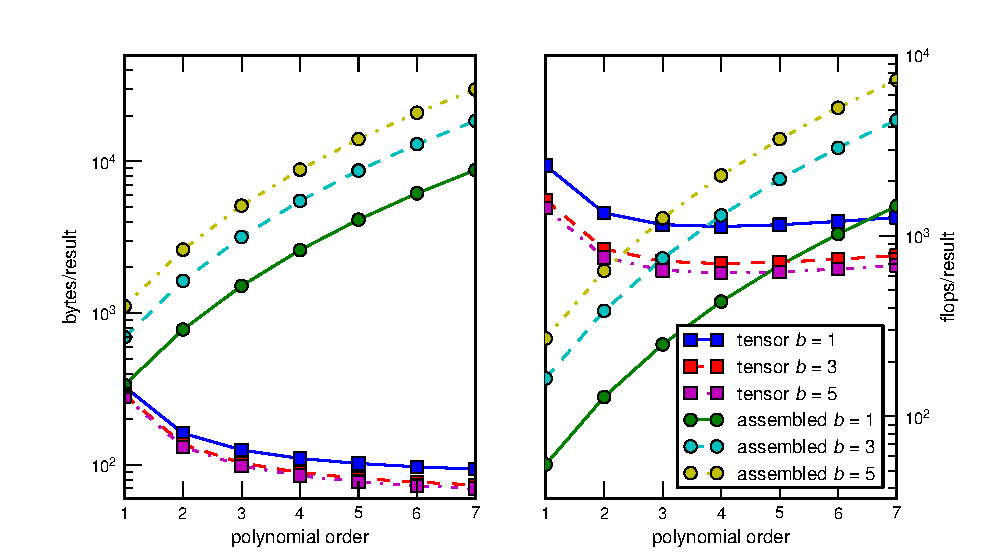
\includegraphics[width=\textwidth]{figures/TensorVsAssembly} \\
  \begin{itemize}
  \item Same linear operator, smaller to not store unassembled
  \item Use local symbolic math or AD, runtime choice of order, precondition with low-order method
  \item Dual order $h$ and $p$ FEM: \url{github.com/jedbrown/dohp}
  \item PETSc: \url{mcs.anl.gov/petsc}
  \end{itemize}
\end{frame}

\begin{frame}[shrink=5]{Automation}
  \begin{itemize}
  \item For unassembled representations, decomposition, and assembly
  \item Continuous weak form: find $u$
    \[ v^T F(u) \sim \int_\Omega v \cdot {\color{green!70!black} f_0(u,\nabla u)}
    + \nabla v \tcolon {\color{green!70!black} f_1(u,\nabla u)} = 0, \qquad \forall v \in \VV_0 \]
  \item Weak form of the Jacobian $J(w)$: find $u$
    \begin{gather*}
      v^T J(w) u \sim \int_\Omega \begin{bmatrix} v^T & \nabla v^T \end{bmatrix}
      {\color{blue} \begin{bmatrix} f_{0,0} & f_{0,1} \\ f_{1,0} & f_{1,1} \end{bmatrix}}
      \begin{bmatrix} u \\ \nabla u \end{bmatrix} \\
      {\color{blue} [f_{i,j}] = \begin{bmatrix} \dfrac{\partial f_0}{\partial u} & \dfrac{\partial f_0}{\partial \nabla u} \\[1em]
          \dfrac{\partial f_1}{\partial u} & \dfrac{\partial f_1}{\partial \nabla u} \end{bmatrix} (w,\nabla w) }
    \end{gather*}
  \item Terms in ${\color{blue} [f_{i,j}]}$ easy to compute symbolically, AD more scalable.
  \item Nonlinear terms ${\color{green!70!black}f_0,f_1}$ usually have the most expensive nonlinearities in the computation of scalars
    \begin{itemize}
    \item Equations of state, effective viscosity
    \item Compute gradient with reverse-mode, store at quadrature points.
    \item Perturb scalars, then use forward-mode to complete the Jacobian.
    \item Flip forward/reverse for action of the adjoint.
    \end{itemize}
  \end{itemize}
\end{frame}

\begin{frame}{Outlook}
  \begin{itemize}
  \item Stabilized continuous FEM is terrible, need to implement DG for transport.
  \item Issues defining conservative normals for slip: all-positive (\eg spline) basis?
  \item Geometric coupling to surface causes delicate stiffness at large time steps.
  \item Visualization should have hooks for solving equations of state.
  \item Need good hierarchical solver diagnostic tools.
  \item Solution transfer after remeshing.
  \item Have active set and semi-smooth Newton for contact, but there are many types of contact and much work to be done.
  \item \emph{Strongly Coupled Solvers with Loosely Coupled Software} \\
    CP76 11:00 tomorrow, Room 304.
  \end{itemize}
\end{frame}

\end{document}
